\documentclass[aspectratio=169]{beamer}

\usepackage[T1]{fontenc}
\usepackage[utf8]{inputenc}
\usepackage[polish]{babel}
\usepackage{graphicx}

\usetheme{Madrid}

\title{Przykładowa analiza danych v2}
\subtitle{Minimalna prezentacja wyników}
\author{Autor pracy magisterskiej}
\date{\today}

\begin{document}

\begin{frame}
    \titlepage
\end{frame}

\begin{frame}{Cel i dane}
    \begin{itemize}
        \item Dane wejściowe znajdują się w pliku CSV.
        \item Python wczytuje dane i tworzy wykres.
        \item LaTeX i Beamer korzystają z tego samego pliku PNG.
    \end{itemize}
\end{frame}

\begin{frame}{Wynik analizy}
    \centering
    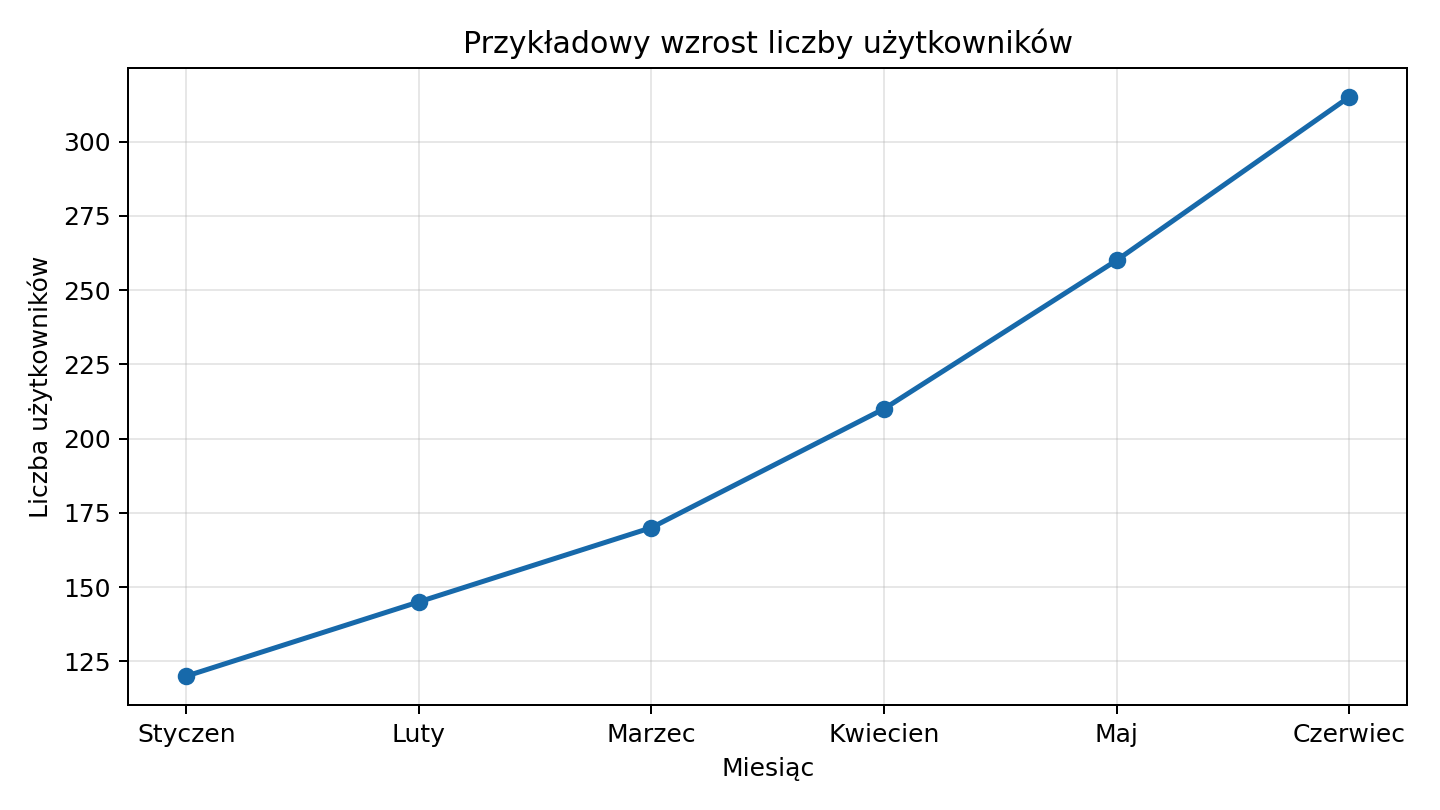
\includegraphics[width=0.82\textwidth]{obrazy/wykres.png}
\end{frame}

\begin{frame}{Twierdzenie Bayesa}
    \begin{block}{Jak dane aktualizują nasze przekonania?}
        \[
            P(H\mid D)
            = \frac{P(D\mid H)\,P(H)}{P(D)}
        \]
    \end{block}

    \begin{itemize}
        \item $P(H)$ opisuje wiedzę początkową o hipotezie.
        \item $P(D\mid H)$ mierzy zgodność hipotezy z danymi.
        \item $P(H\mid D)$ jest zaktualizowanym prawdopodobieństwem hipotezy.
    \end{itemize}
\end{frame}

\end{document}
